% !TEX encoding = UTF-8 Unicode
\documentclass[titlepage]{report}
%\documentclass[fontsize=12pt]{article}

\usepackage[utf8]{inputenc}
\usepackage[T1]{fontenc}
\usepackage{illcmolthesis}
\usepackage[a4paper, margin=1.08in]{geometry}
\usepackage{amsmath}
\usepackage{amsfonts}
\usepackage{amssymb}
\usepackage[mathscr]{eucal}
\usepackage{enumitem}
\usepackage{mathtools}
\usepackage{IEEEtrantools}
\usepackage[backend=bibtex]{biblatex}
\usepackage{indentfirst}
\usepackage{physics}
\usepackage{bm}
\usepackage{mathtools}
\usepackage{etoolbox}
\usepackage{xifthen}
\usepackage{ulem}
\usepackage{titlesec}
\usepackage{hyperref}
\usepackage[ruled, linesnumbered, noalgohanging]{algorithm2e}

\addbibresource{references.bib}

\newcounter{theorem}
\newcounter{lemma}

\newcommand\where[1][\big]{\:#1\vert\:}
\DeclareMathOperator*{\argmin}{arg\,min}
\DeclareMathOperator*{\argmax}{arg\,max}
\DeclareMathOperator{\softmax}{softmax}
\DeclareMathOperator{\score}{score}
\DeclareMathOperator{\aln}{align}
\DeclareMathOperator{\relu}{ReLU}
\DeclareMathOperator{\CTM}{CTM}
\DeclareMathOperator{\BDM}{BDM}

\makeatletter
\newcommand{\RemoveAlgoNumber}{\renewcommand{\fnum@algocf}{\AlCapSty{\AlCapFnt\algorithmcfname}}}
\newcommand{\RevertAlgoNumber}{\algocf@resetfnum}
\makeatother

%\setul{5pt}{.4pt}

\newenvironment{def*}[1][]
	{%
	\par\addvspace{9pt}%
	\noindent%
	\uline{\textbf{Definition%
	\ifthenelse{\isempty{#1}}%
		{}%
		{ (#1)}%
	}}%
	\hspace{5pt}%
	\ignorespaces%
	}
	{%
	\par\addvspace{9pt}%
	}

\newenvironment{theorem}[1][]
	{%
	\stepcounter{theorem}%
	\par\addvspace{9pt}%
	\noindent%
	\uline{\textbf{Theorem \thetheorem%
	\ifthenelse{\isempty{#1}}%
		{}%
		{ (#1)}%
	}}%
	\hspace{5pt}%
	\ignorespaces%
	}
	{%
	\par\addvspace{9pt}%
	}

\newenvironment{proof}[1][]
	{%
	\par\addvspace{9pt}%
	\noindent%
	\uline{\textbf{Proof%
	\ifthenelse{\isempty{#1}}%
		{}%
		{ (#1)}%
	}}%
	\hspace{5pt}%
	\ignorespaces%
	}
	{%
	\hfill%
	$\square$%
	\par\addvspace{9pt}%
	}

\newenvironment{lemma}[1][]
	{%
	\stepcounter{theorem}%
	\par\addvspace{9pt}%
	\noindent%
	\uline{\textbf{Lemma \thetheorem%
	\ifthenelse{\isempty{#1}}%
		{}%
		{ (#1)}%
	}}%
	\hspace{5pt}%
	\ignorespaces%
	}
	{%
	\par\addvspace{9pt}%
	}

\newenvironment{corollary}[1][]
	{%
	\stepcounter{theorem}%
	\par\addvspace{9pt}%
	\noindent%
	\uline{\textbf{Corollary \thetheorem%
	\ifthenelse{\isempty{#1}}%
		{}%
		{ (#1)}%
	}}%
	\hspace{5pt}%
	\ignorespaces%
	}
	{%
	\par\addvspace{9pt}%
	}

\newenvironment{corollary*}[1][]
	{
	\par\addvspace{9pt}%
	\noindent%
	\uline{\textbf{Corollary%
	\ifthenelse{\isempty{#1}}%
		{}%
		{ (#1)}%
	}}%
	\hspace{5pt}%
	\ignorespaces%
	}
	{%
	\par\addvspace{9pt}%
	}

\newenvironment{example*}[1][]
	{
	\par\addvspace{9pt}%
	\noindent%
	\uline{\textbf{Example%
	\ifthenelse{\isempty{#1}}%
		{}%
		{ (#1)}%
	}}%
	\hspace{5pt}%
	\ignorespaces%
	}
	{%
	\par\addvspace{9pt}%
	}

\titlespacing{\section}{0pt}{24pt}{18pt}

\hypersetup{
	colorlinks = true,
	urlcolor = blue
}

\title{THESIS TITLE}
\author{Krsto Proroković}
\birthdate{March 12, 1993}
\birthplace{Kotor, Montenegro}
\defensedate{Date of the defense goes here}
\supervisor{Dr Germán Kruszewski}
\supervisor{Dr Elia Bruni}
\committeemember{Committee goes here}

\setlength{\parindent}{12pt}

\begin{document}

\maketitle
\RemoveAlgoNumber

\begin{abstract}
Abstract goes here
\end{abstract}

\chapter*{Acknowledgents}

\tableofcontents

\chapter{Introduction}

\chapter{Background}

\section{Locally k-testable languages}

Fix an alphabet $\mathcal{A} = \{ a_1, a_2, \ldots, a_n \}$. An $SL_k$ definition is just a set of blocks of $k$ adjacent symbols (called $k$-factors) drawn from the alphabet. A string satisfies the description if and only if every $k$-factor that occurs in the string is licensed by the definition. We can see $k$-factors as atomic properties of strings: a string satisfies a $k$-factor if and only if that factor occurs somewhere in the string. Then, we can build descriptions as propositional formulas over these atoms. We will call these formulas $k$-expressions. A $k$-expression defines the set of all strings that satisfy it. A language that is defined in this way is called a locally $k$-testable ($LT_k$) language.
\par
A scanner for an $LT_k$ language contains a table in which it records, for every k-factor over the alphabet, whether or not that $k$-factor has occurred somewhere in the string. It then feeds this information into a Boolean network which implements some $k$-expression. When the end of the string is reached, the automaton accepts or rejects the string depending on the output of the network.

\begin{center}
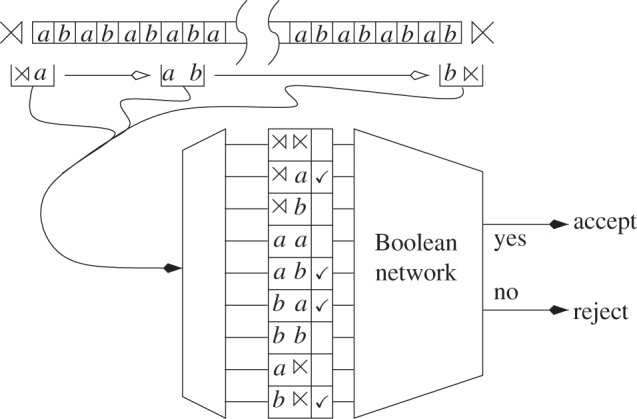
\includegraphics[width=80mm]{locally_k-testable.jpg}
\end{center}

\section{Recurrent Neural Networks}

Recurrent neural networks (RNNs) \cite{rumelhart1985learning} are parametric models of computation for processing sequences loosely inspired by biological neural networks. They found applications in handwriting recognition [reference], speech recognition [reference], machine translation [reference], etc. In this section we provide an introduction to RNNs and ... For a more detailed treatment we point the reader to \cite{graves2012supervised}.

\subsection{Vanilla Recurrent Neural Networks}

We start with a simple vanilla RNN model. A vanilla RNN is given with the following parameters:

\begin{itemize}[itemsep = -2pt]
\item Input to hidden connection weights $W_x \in \mathbb{R}^{d_h \times d_x}$
\item Hidden to hidden connection weights $W_h \in \mathbb{R}^{d_h \times d_h}$
\item Bias term $b_h \in \mathbb{R}^{d_h}$
\item Activation function $\phi: \mathbb{R} \to \mathbb{R}$
\item Hidden to output connection weights $W_y \in \mathbb{R}^{d_y \times d_y}$
\item Bias term $b_y \in \mathbb{R}^{d_y}$
\item Initial hidden state $h^{(0)} \in \mathbb{R}^{d_h}$ (usually set to zero vector)
\end{itemize}

\noindent
Connection weights model the strength of synapses and activation function models neuronal firing \cite{llinas2008neuron}. Most commonly used activation functions are sigmoid $\sigma(x) = 1 / (1 + \exp(-x))$, hyperbolic tangent $\tanh(x) = (\exp(x) - \exp(-x)) / (\exp(x) + \exp(-x))$ and rectified linear unit $\relu(x) = \max \{ 0, x \}$.

%\begin{IEEEeqnarray*}{rcl}
%\text{sigmoid} \: \sigma(z) &= \frac{1}{1 + \exp(-z)} & 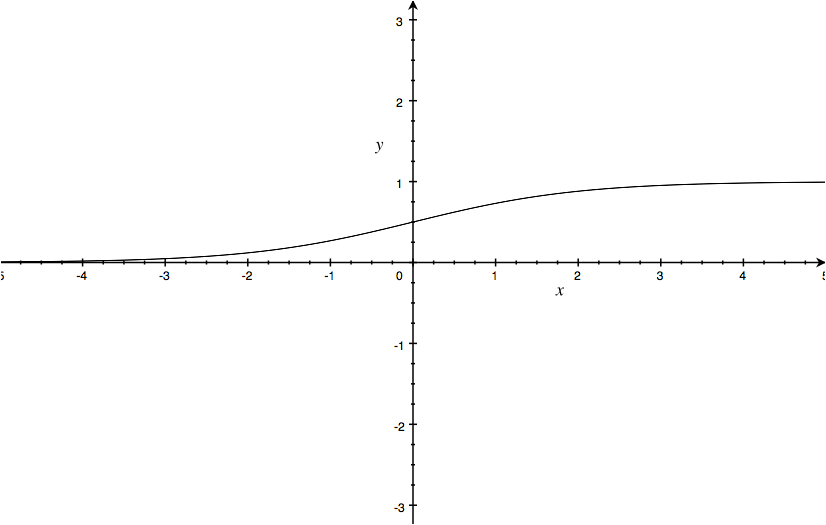
\includegraphics[width=60mm]{sigma} \\
%\text{sigmoid} \: \sigma(z) &= \frac{1}{1 + \exp(-z)} & 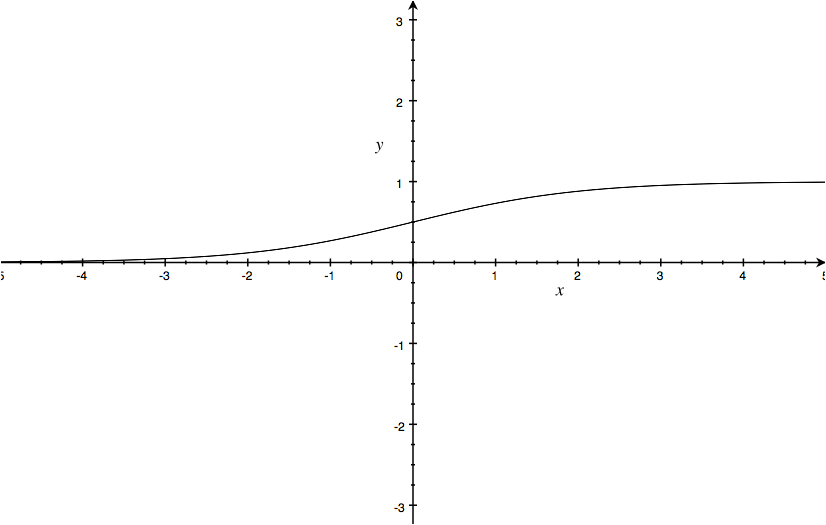
\includegraphics[width=60mm]{sigma}
%\end{IEEEeqnarray*}

\begin{center}
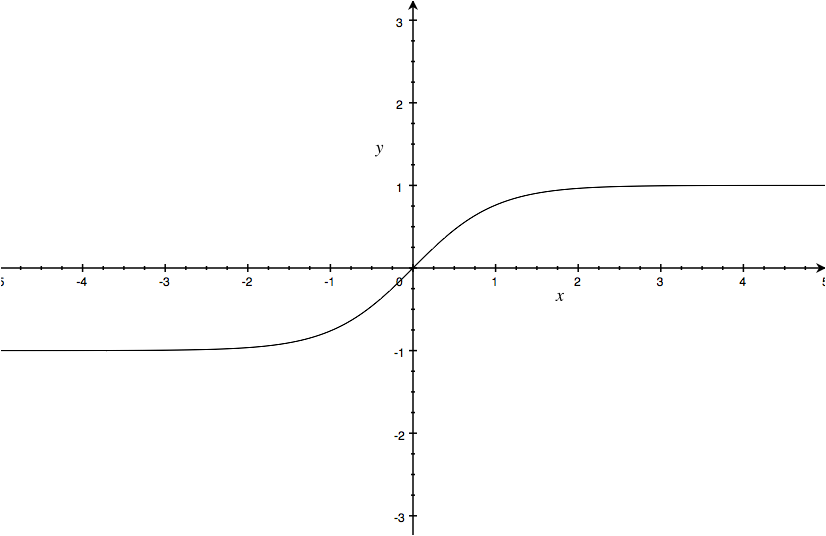
\includegraphics[width=60mm]{tanh} \\
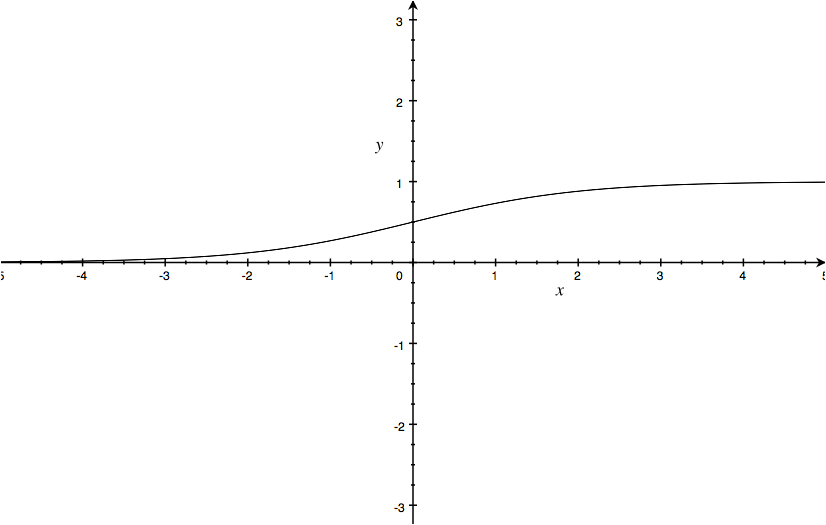
\includegraphics[width=60mm]{sigma} \\
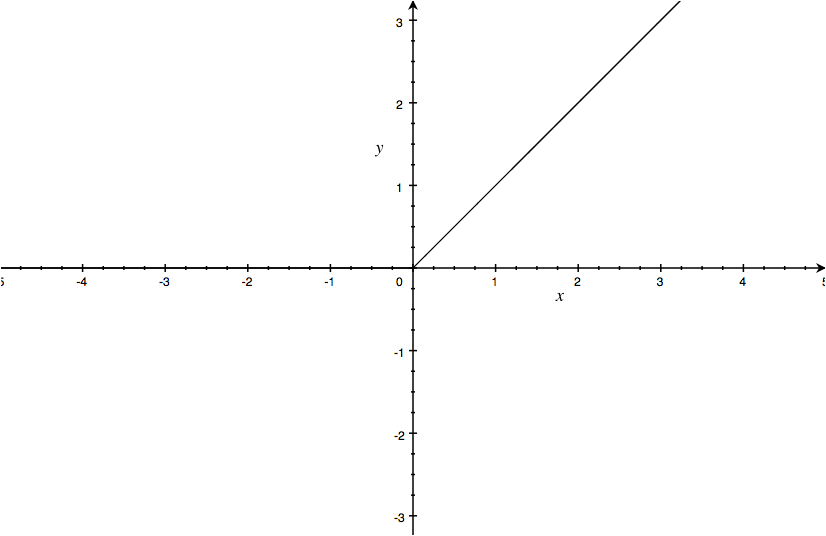
\includegraphics[width=60mm]{relu}
\end{center}

\noindent
The computation is performed in the following way: for $t = 1, 2, \ldots, T$
\begin{align*}
h^{(t)} &= \boldsymbol{\phi} \left( W_h h^{(t - 1)} + W_x x^{(t)} + b_h \right) \\
y^{(t)} &= \softmax \left( W_y h^{(t)} + b_y \right)
\end{align*}

\noindent
where $\boldsymbol{\phi}(v)_i = \phi(v_i)$ and $\softmax(v)_i = \exp(v_i) / \sum_j \exp(v_j)$. 

\begin{center}
RNN figure goes here.
\end{center}

\noindent
Note that components of $y^{(t)}$ sum up to one, so we can interpret it as a probability distribution. Here we will be mostly interested in sequence classification, i.e. we will only care about $y^{(T)}$.

\begin{example*}
Consider a vanilla RNN given with the following parameters
\begin{equation*}
W_x = \begin{bmatrix} 3 & -1 & 0 \\ 0 & 0 & 2 \end{bmatrix} \quad
W_h = \begin{bmatrix} 1 & 0 \\ 0 & 1 \end{bmatrix} \quad
b_h = \begin{bmatrix} 0 \\ 0 \end{bmatrix} \quad
W_y = \begin{bmatrix} 1 & 0 \\ 0 & 1 \end{bmatrix} \quad
b_y = \begin{bmatrix} 0 \\ 0 \end{bmatrix}
\end{equation*}
\end{example*}

\noindent
and $\phi(z) = z$. It is easy to see that $y_1^{(T)} < y_2^{(T)}$ if and only if $\sum_t ( 3 x_1^{(t)} - x_2^{(t)} ) < \sum_t 2 x_3^{(t)}$. Note that in this case $h^{(t)}$ accumulates the results of the computation on the input encountered so far. \\
%$h^{(t)} = \sum_t$ ... \\

While the previous example displays a rather simple function, vanilla RNNs are universal in the sense that any function computable by a Turing machine can be computed by such a network [reference Siegelmann and Sontag].

We can also stack several RNN cells in order to exploit compositionality and obtain more powerful RNNs. Such RNNs are called multilayer or deep RNNs. The computation performed by an $L$ layer vanilla RNN is given with
\begin{align*}
\mathbf{h}_1^{(t)} &= \boldsymbol{\phi} \left( \mathbf{W}^{\mathbf{h}_1 \mathbf{h}_1} \mathbf{h}_1^{(t - 1)} + \mathbf{W}^{\mathbf{x} \mathbf{h}_1} \mathbf{x}^{(t)} + \mathbf{b}^{\mathbf{h}_1} \right) \\
\mathbf{h}_2^{(t)} &= \boldsymbol{\phi} \left( \mathbf{W}^{\mathbf{h}_2 \mathbf{h}_2} \mathbf{h}_2^{(t - 1)} + \mathbf{W}^{\mathbf{x} \mathbf{h}_2} \mathbf{x}^{(t)} + \mathbf{b}^{\mathbf{h}_2} \right) \\
& \enspace \vdots \\
\mathbf{h}_L^{(t)} &= \boldsymbol{\phi} \left( \mathbf{W}^{\mathbf{h}_L \mathbf{h}_L} \mathbf{h}_L^{(t - 1)} + \mathbf{W}^{\mathbf{x} \mathbf{h}_L} \mathbf{x}^{(t)} + \mathbf{b}^{\mathbf{h}_L} \right) \\
\mathbf{y}^{(t)} &= \softmax \left( \mathbf{W}^{\mathbf{h}_L \mathbf{y}} \mathbf{h}_L^{(t - 1)} + \mathbf{b}^{\mathbf{y}} \right)
\end{align*}
Observe that we will need $L$ initial states $\mathbf{h}_1^{(0)}, \mathbf{h}_2^{(0)}, \ldots, \mathbf{h}_L^{(0)}$.

\subsection{Backpropagation Through Time and Vanishing Gradient}

In practice we need to estimate the parameters of RNN from the data. The way this is done is by minimising the average of a certain loss function which measures how far are the outputs of the network from actual data. Suppose that we are given a dataset $\mathcal{D} = \{ (\mathbf{x}_1, \mathbf{y}_1), (\mathbf{x}_2, \mathbf{y}_2), \ldots, (\mathbf{x}_n, \mathbf{y}_n) \}$. The quantity that we are supposed to minimise is

\begin{equation*}
\mathcal{L}(\theta) = \frac{1}{n} \sum_{i = 1}^n \ell(\mathbf{y}_i, \mathbf{\hat{y}}_i)
\end{equation*}
where $\theta$ are parameters of the network and $\mathbf{\hat{y}}_i$ is the output of the network on input $\mathbf{x}_i$. The loss function that we will use here is the cross entropy loss given with
\begin{equation*}
\ell(\mathbf{y}, \mathbf{\hat{y}}) = - \sum_i y_i \log \hat{y}_i \: .
\end{equation*}

\noindent
In order to minimise the loss function we need to calculate its gradient with respect to the parameters of the network. This is achieved by Backpropagation Through Time algorithm \cite{werbos1990backpropagation}.

Unfortunately, for vanilla RNNs this does not solve the optimisation problem. The reason is that is that the gradient of the loss function may vanish or explode over many time steps. This problem has been studied independently by separate researchers [Hochreiter][Bengio]. For survey see [paper by Pascanu and Bengio].

The problem of exploding gradient can be solved by gradient clipping: if the norm of the gradient exceeds a certain threshold, then normalise it and multiply it by that threshold.
However, the vanishing gradient remains a problem for vanilla RNNs which makes their optimisation difficult in practice.

\subsection{Long-Short Term Memory Networks}

One way to deal with vanishing gradient is to use gated RNNs whose connection weights may change at each time step. Multiplicative gates allow RNNs to control the way information is stored and retrieved. Thus, they are able to create paths through time that have derivatives that neither vanish nor explode. Gates in RNNs can be seen as differentiable version of logic gates in digital circuits.
\par
Long short term memory (LSTM) networks \cite{hochreiter1997long} 
%... Apart from hidden state $h^{(t)}$ LSTM uses 
use additional memory cell $c^{(t)}$ apart from $h^{(t)}$. Here we will be using standard LSTM architecture introduced in \cite{gers1999learning} which uses four gates: forget gate $f^{(t)}$, input gate $i^{(t)}$, output gate $o^{(t)}$ and input modulation gate $g^{(t)}$. Its cell is described by the following set of equations
\begin{IEEEeqnarray*}{cl}
\begin{bmatrix} f^{(t)} \\ i^{(t)} \\ o^{(t)} \\ g^{(t)} \end{bmatrix} &= W_x x^{(t)} + W_h h^{(t)} + b \\
c^{(t)} &= \sigma(f^{(t)}) \odot c^{(t-1)} + \sigma(i^{(t)}) \odot \tanh(g^{(t)}) \\
h^{(t)} &= \sigma(o^{(t)}) \odot \tanh(c^{(t)})
\end{IEEEeqnarray*}

\noindent
where $\odot$ is component-wise or Hadamard product.

\begin{center}
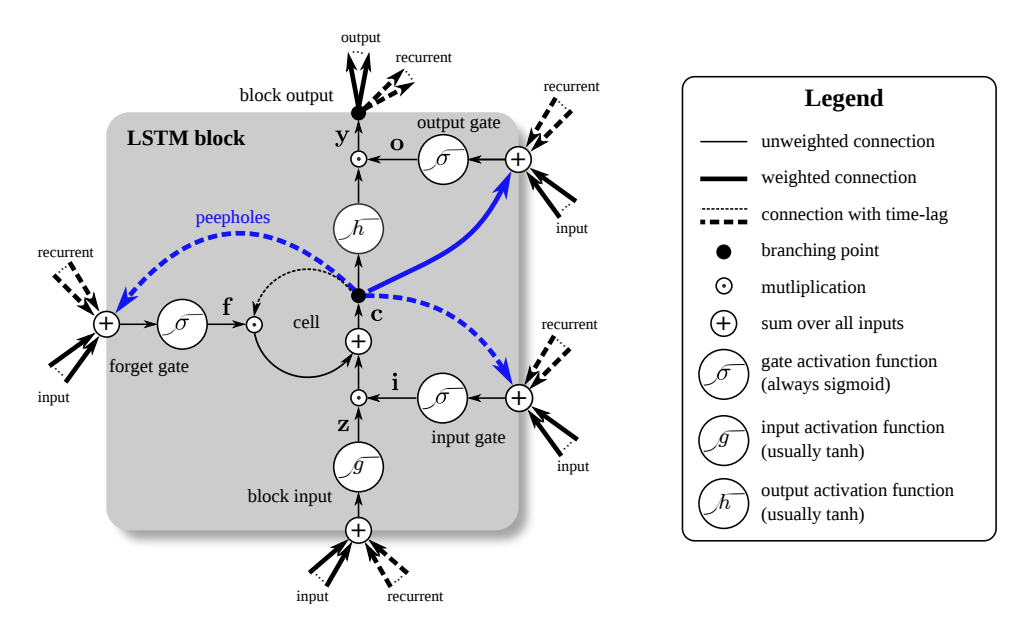
\includegraphics[width=120mm]{lstm}
\end{center}

Just like vanilla RNN cells, LSTM cells can be stacked in order to obtain more powerful multilayer LSTM networks.

LSTM networks have been successfully applied in many contexts such as handwriting recognition [reference] and generation, language modeling [reference], machine translation [reference], image captioning [reference], parsing [reference], etc.

\subsection{Gated Recurrent Units}

Another gated recurrent architecture frequently used in practice are Gated Recurrent Units (GRU) \cite{cho2014learning}. Unlike LSTM, GRU gets rid of memory cell $c^{(t)}$ by combining input and forget gates into a single one. The GRU cell is described by the following set of equations
\begin{IEEEeqnarray*}{cl}
r^{(t)} &= \sigma(W_{xr} x_t + W_{hr} h^{(t-1)} + b_r) \\
z^{(t)} &= \sigma(W_{xr} x_t + W_{hz} h^{(t-1)} + b_z) \\
n^{(t)} &= \tanh(W_{xn} x_t + r_t (W_{hn} h^{(t-1)} + b_n)) \\
h^{(t)} &= (1 - z_t) n_t + z_t h_{t-1}
\end{IEEEeqnarray*}

\begin{center}
GRU figure goes here.
\end{center}

Again, GRU cells can be stacked, yielding multilayer GRU networks.

\subsection{One-hot and Dense Encodings}

Note that RNNs work exclusively with numerical data, i.e. real numbers. Suppose that we are given an alphabet $\mathcal{A} = \{ a_1, a_2, \ldots a_k \}$. One way to encode it would be to map each $a_i$ to $i$. However, this is not a good encoding as the network would need to learn that there is no ordering between alphabet elements. A better way to encode the alphabet that avoids this problem is to assign a one-hot vector to every element of the alphabet, i.e.
\begin{equation*}
a_1 \mapsto \begin{bmatrix} 1 \\ 0 \\ \vdots \\ 0 \end{bmatrix} \quad
a_2 \mapsto \begin{bmatrix} 0 \\ 1 \\ \vdots \\ 0 \end{bmatrix} \quad
\ldots \quad
a_k \mapsto \begin{bmatrix} 0 \\ 0 \\ \vdots \\ 1 \end{bmatrix}
\end{equation*}

One problem with this encoding is that $k$ may be huge while one-hot vectors remain sparse. For example, in natural language processing $k$ would be the number of words which is usually several tens of thousands. This problem is solved by using embedding layer which learns to map alphabet elements to dense, low-dimensional encodings.

\subsection{Attention Mechanism}

When processing the input, RNNs store all the memory in the hidden state. However, it may be hard to compress potentially long input in a single context vector.
This could definitely be an issue if the hidden state is passed as input to another network which is common in sequence to sequence learning. For example, the family of models used for machine translation has one RNN called encoder to process the input in one language and pass it to the other RNN called decoder which is supposed to output a sequence in a different language.

Attention mechanism allows us to obtain a distribution on part of the input provided so far and focus on certain parts of it in a way we humans do. The attentional hidden state is defined as
\begin{equation*}
\widetilde{h}^{(t)} = \tanh(W_c [c^{(t)}; h^{(t)}])
\end{equation*}
where $c^{(t)}$ is the context vector and $[ ; ]$ denotes concatenation. We will be using an attention model in which the alignment vector $a^{(t)}$ is obtained by comparing the current hidden state $h^{(t)}$ with each source hidden state $\bar{h}^{(s)}$

\begin{equation*}
a^{(t)} = \aln (h^{(t)}, \bar{h}^{(s)}) = \softmax(\score(h^{(t)}, \bar{h}^{(s)})) \:.
\end{equation*}

\begin{center}
Attention figure goes here.
\end{center}

\chapter{Experiments and Results}

\normalem
\printbibliography

\end{document}